\documentclass[handout]{beamer}
\usetheme{Antibes}
\usecolortheme{beaver}

% \usepackage{beamerthemesplit}
\usepackage{pgfpages}
\usepackage{verbatim}
\usepackage{fancybox}
\usepackage{algorithm}
\usepackage{amsmath}
\usepackage{amsthm}
\usepackage{algpseudocode}
\usepackage{algorithmicx}% http://ctan.org/pkg/algorithmicx
\usepackage{lipsum}% http://ctan.org/pkg/lipsum
\usepackage{xifthen}% http://ctan.org/pkg/xifthen
\usepackage{needspace}% http://ctan.org/pkg/needspace
\usepackage{hyperref}% http://ctan.org/pkg/hyperref
\usepackage{tikz}
\usepackage{mathptmx}
\usepackage[scaled=.90]{helvet}
\usepackage[T1]{fontenc}

% Multiple pages...
%\pgfpagesuselayout{4 on 1}
%\pgfpagesuselayout{4 on 1}[letterpaper,border shrink=5mm]


\title[Merging Modern Cryptography with CCN]{Merging Modern Cryptography with CCN}
\institute[RIT - UCI]{RIT - UCI}
\date{\today}
%\subtitle{}
\author{Christopher A. Wood \\ {\tt www.christopher-wood.com}}
%\institute[]{}
\date{\today}

\begin{document}

%%%%%
%%
%% Resource link: http://www.math-linux.com/spip.php?article77
%%
%%%%

\begin{frame}
	\titlepage
\end{frame}

\begin{frame}
	\frametitle{Agenda}
	\tableofcontents
\end{frame}

%%% outline
% CCN general usage
% 	Terminology (CS, FIB, PIT)
% 	Flow of traffic (flow control)
% 	Signatures and routing (it is \emph{not} based on the content inside the packets, but on the path the routers/notes set up with routing protocols)
% 	View in mobile networks
% Protecting CCN traffic
% 	Pick any scheme you want (hybrid sk/pk)
% 	ABE for more fine-grained access control
% 	Steady-state broadcast encryption for fine-grained control (DESCRIBE)
% 	Proxy re-encryption (good: individualized, bad: re-encryption key needed before hand, installed at mission time?)
% Functional Encryption
% 	Start with IBE!
% 	Idea: decrypt ONLY if a certain functionality passes
% 	ABE: has attributes, HVE: dot product is 1, etc etc
% 	Useful for specifying different types of (aka more flexible) access control, rather than having it be based on possession of a simple secret key

\section{Content-Centric Networking Fundamentals}
\begin{frame}
	\frametitle{CCN Overview}
	\begin{itemize}
		\item Content-centric networking flips around the host-based model of the Internet architecture
		\begin{itemize}
			\item \emph{Content names}, rather than content locations, become addressable. 
			\item The network is permitted to store (cache) content that is in high demand
			\item End result: less traffic to/from the content's original source, better usage of network resources, less latency, etc etc.
		\end{itemize}
	\end{itemize}
\end{frame}

\begin{frame}
	\frametitle{CCN Overview (continued)}
	How is data actually retrieved? 
	\begin{itemize}
		\item A consumer $C$ sends out an \emph{interest} for content they desire.
		\item A router $R_i$ use the information in their forwarding information base (FIB) table and data in cached in their content store (CS) to handle incoming interests:
		\begin{enumerate}
			\item If content with the same name matches what's stored in the CS, return that content
			\item Else, store the interest in their pending interest table (PIT) (including the downstream router $R_{i-1}$ or consumer $C$ that made the request), and forward the request upstream to the next router $R_{i+1}$ based on their FIB.
			\item FIBs are configured using protocol similar to OSPF
		\end{enumerate}
		\item Once the interest is satisfied in $R_i$, the PIT entry is cleared, the content is cached, and the data is sent downstream to $C$ or $R_{i-1}$. 
 	\end{itemize}
\end{frame}

\begin{frame}
	\frametitle{Interest Format}
	\begin{itemize}
		\item Interests are similar to URLs: 
		\begin{center}
			{\tt ccnx://rit/gccis/cs/spr/ramsey\_survey}
		\end{center}
		\item The {\tt /} character is a delimeter that separates name \emph{components}
		\item A component can be \emph{anything}, including binary data (e.g. ciphertext)
		\item Interests are matched to providers in FIBs using a standard longest-prefix rule (to my knowledge, interests in CSs must match completely)
	\end{itemize}
\end{frame}

%% TODO: images of this happening 
\begin{frame}
	\frametitle{CCN in Action - \#1}
	\begin{figure}[h]
		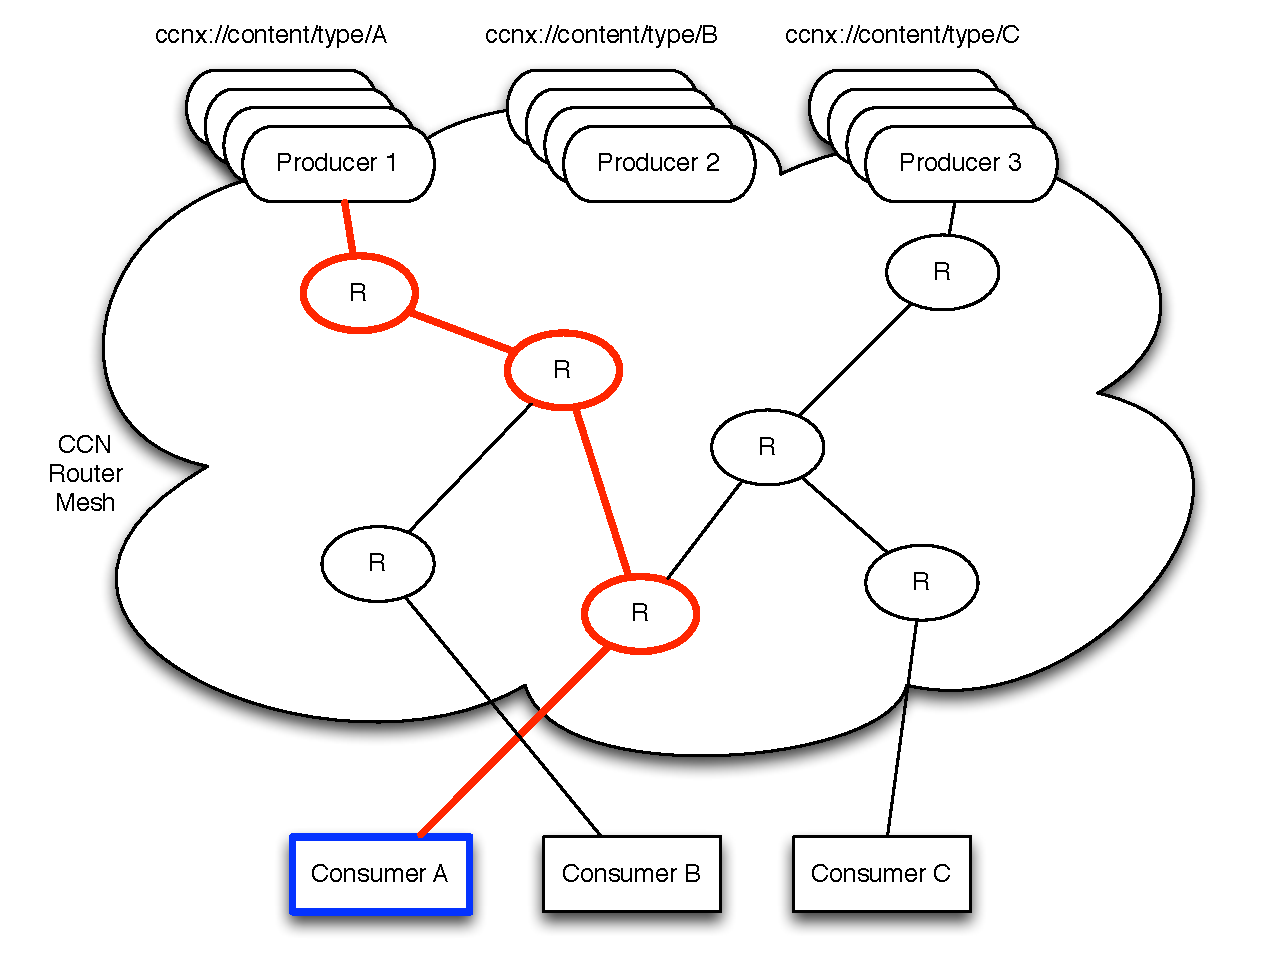
\includegraphics[scale=0.4]{ccn_img1.pdf}
	\end{figure}
\end{frame}

\begin{frame}
	\frametitle{CCN in Action - \#2}
	\begin{figure}[h]
		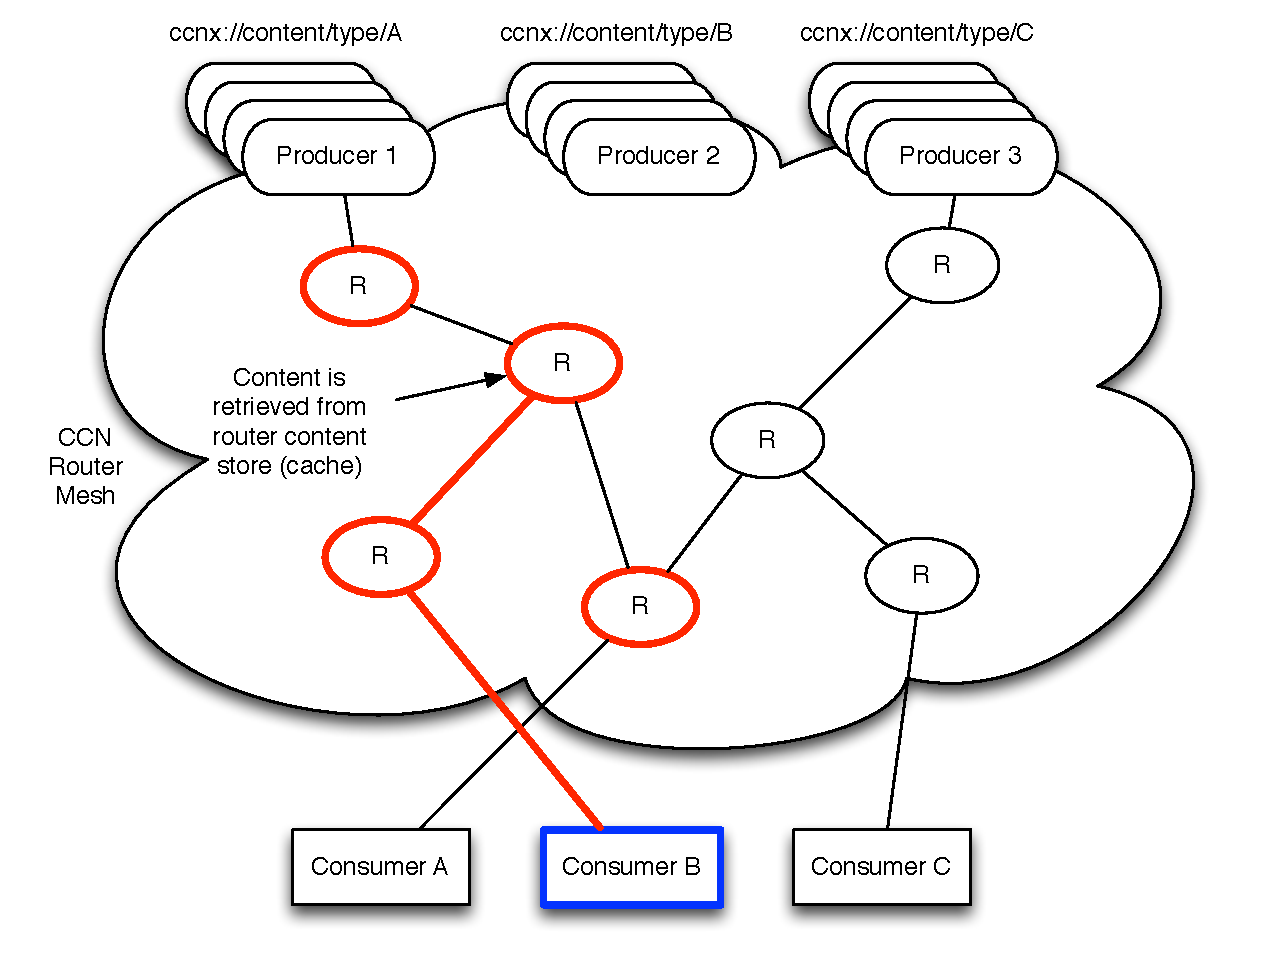
\includegraphics[scale=0.4]{ccn_img2.pdf}
	\end{figure}
\end{frame}

\begin{frame}
	\frametitle{CCN in Action - \#3}
	\begin{figure}[h]
		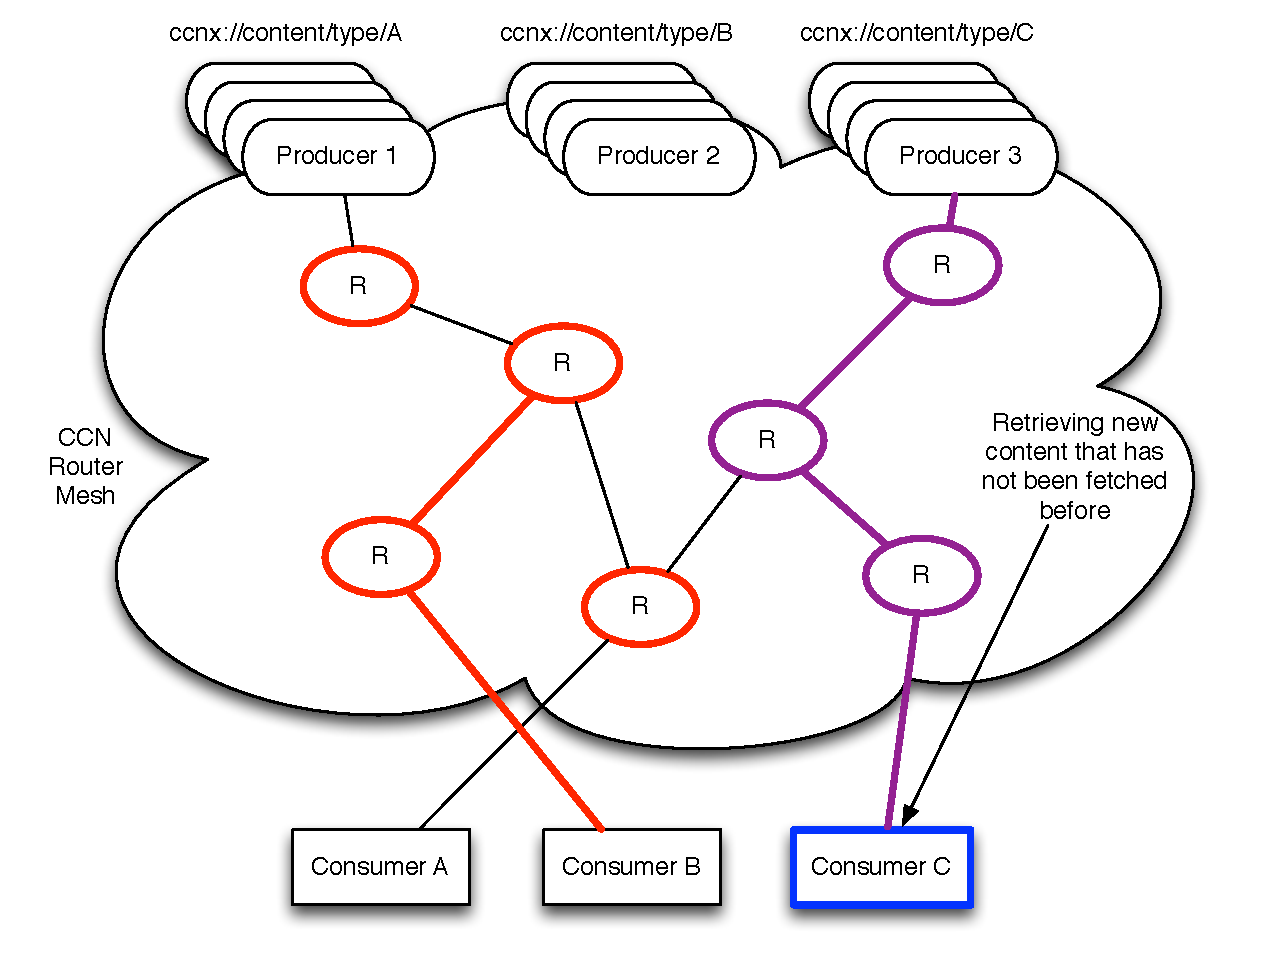
\includegraphics[scale=0.4]{ccn_img3.pdf}
	\end{figure}
\end{frame}

\begin{frame}
	\frametitle{CCN in Action - \#4}
	\begin{figure}[h]
		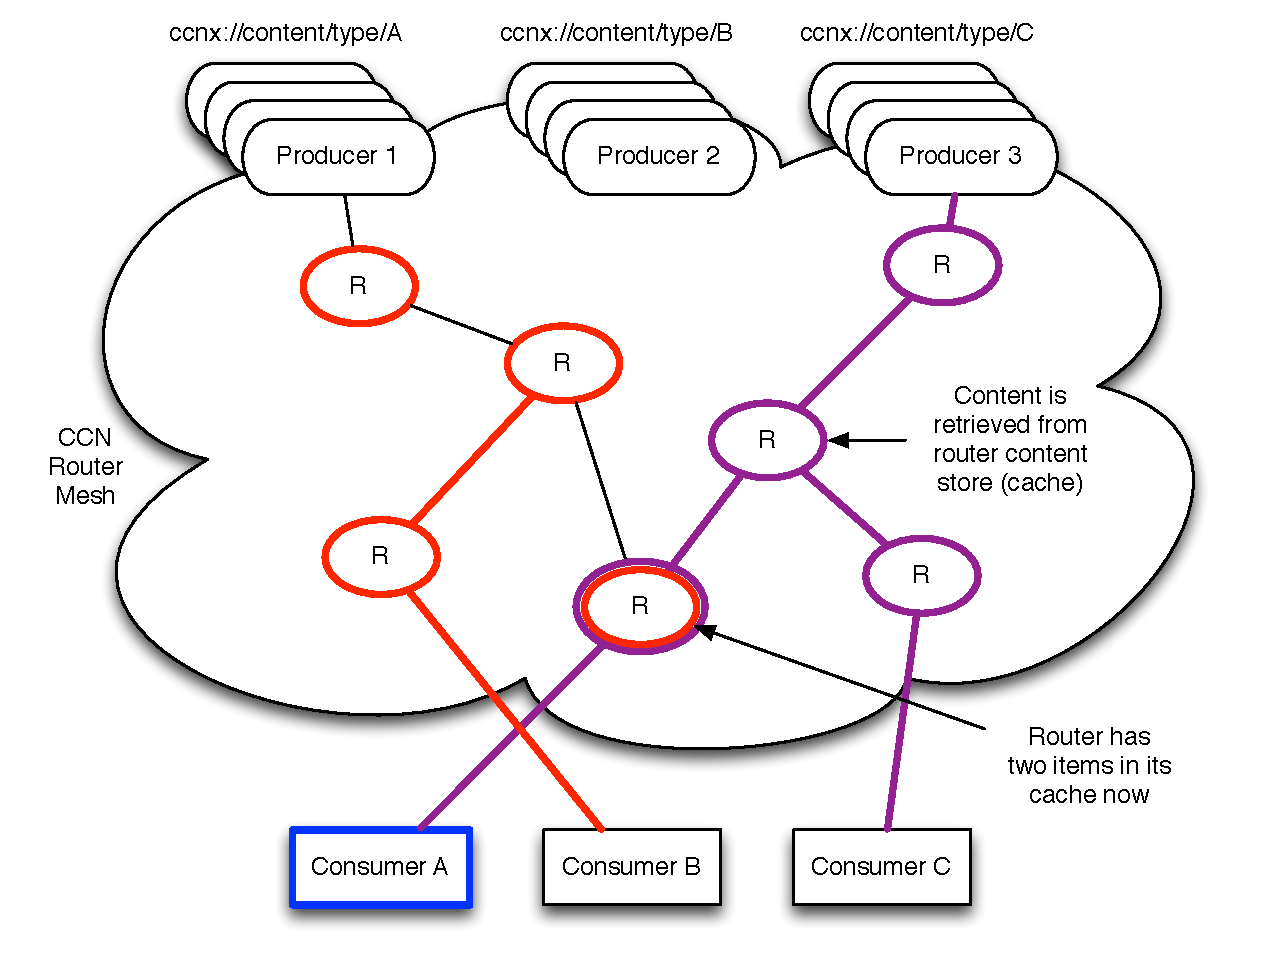
\includegraphics[scale=0.4]{ccn_img4.pdf}
	\end{figure}
\end{frame}

\begin{frame}
	\frametitle{Notes about the Content and Cache}
	Content details:
	\begin{itemize}
		\item By default, \emph{every} of data is signed by its consumer
		\begin{itemize}
			\item Good: provides separation from security and the channel through which data is routed, and consumers can verify the validity of the content if they know the public information about the producer
			\item ``Bad'': In an ideal world, every router would verify the signature of every piece of content it receives from an upstream router - this is a computationally infeasible task.
		\end{itemize}
	\end{itemize}
	\medskip

	Cache details:
	\begin{itemize}
		\item LRU is the default policy used in CCN (and CCNx, the open source platform)
		\item The network engineer is free to select cache replacement policy to suit the type of traffic
	\end{itemize}
\end{frame}

\begin{frame}
	\frametitle{Flow Control}
	\begin{center}
		\textbf{All traffic obeys the principle of flow control}
	\end{center}
	\begin{itemize}
		\item Interests that go ``into'' the network are matched with content that comes ``out of'' the network
		\item Routing decisions \emph{are not made} based upon the content itself, but rather:
		\begin{enumerate}
			\item Upstream traffic is routed based on the contents of the FIB (established with a routing protocol)
			\item Downstream traffic is routed based on the interface from which interests were received
		\end{enumerate}
	\end{itemize}
\end{frame}

\begin{frame}
	\frametitle{Negative Aspects of CCN}
	Denial of Service (DoS) attacks are plentiful:
	\begin{itemize}
		\item Malicious consumers can send out fake/invalid interests (i.e. those that won't match an entry in any FIB) that steal the router's computational resources
		\begin{itemize}
			\item There are solutions, such as exponential backoff heuristics to gradually accept less and less traffic on interfaces providing fake interests.
		\end{itemize}
		\item Content stores can also be flooded with fraudulent data
		\begin{itemize}
			\item Recall, signatures are \emph{not} always verified at the routers
			\item A malicious consumer can produce content that match an interest in a router's PIT but that is also invalid
			\begin{itemize}
				\item One solution: consumers verify the signature, realize the data is invalid, and re-send an interest by specifying that content be excluded from the response (forces router to request new data from legitimate producer)
			\end{itemize}
		\end{itemize}
	\end{itemize}
\end{frame}

\begin{frame}
	\frametitle{Worst of Both Worlds}
	Two-pronged attacks: malicious producers and consumers
	\begin{itemize}
		\item Attackers coordinate to flood with both invalid interests and valid (but fraudulent!) returned content that will be stored in the CS
		\item This leaves no room for legitimate data needed by other honest consumers
	\end{itemize}
\end{frame}

%%% TODO; crypto now

\section{Proxy Re-Encryption}
\begin{frame}
	\frametitle{Changing Gears}
	\begin{center}
	A closer look at some new cryptographic primitives
	\end{center}
\end{frame}

\begin{frame}
	\frametitle{An Introduction to Proxy Re-Encryption}
	Consider the following scenario...
	\begin{figure}[h]
		\includegraphics[scale=0.55]{pre_overview.pdf}
	\end{figure}
\end{frame}

\begin{frame}
	\frametitle{An Introduction to Proxy Re-Encryption (continued)}
	\begin{figure}[h]
		\includegraphics[scale=0.6]{pre_overview_2.pdf}
	\end{figure}
\end{frame}

\begin{frame}
	\frametitle{An Introduction to Proxy Re-Encryption (continued)}
	\begin{figure}[h]
		\includegraphics[scale=0.6]{pre_overview_3.pdf}
	\end{figure}
\end{frame}

\begin{frame}
	\frametitle{An Introduction to Proxy Re-Encryption (continued)}
	\begin{figure}[h]
		\includegraphics[scale=0.6]{pre_overview_4.pdf}
	\end{figure}
\end{frame}

\begin{frame}
	\frametitle{An Introduction to Proxy Re-Encryption (continued)}
	\begin{figure}[h]
		\includegraphics[scale=0.6]{pre_overview_5.pdf}
	\end{figure}
\end{frame}

\begin{frame}
	\frametitle{Proxy Re-Encryption Overview} 
	\begin{itemize}
		\item Proxy Re-Encryption (PRE) has been studied since the idea was first introduced at Eurocrypt in 1998.
		\item It can be constructed from pairings (see the Green-Ateniese identity-based PRE scheme) or clever combinations of ``hashed''ElGamal public-key encryption and Schnorr signature schemes
		\begin{itemize}
			\item Basically, the signature scheme is used to protect a token passed between parties, ElGamal encryption is used to transform plaintext masks encrypted with one public key to another, and hashes are used to hide secret keys
		\end{itemize}
	\end{itemize}
\end{frame}

\begin{frame}
	\frametitle{PRE Description}
	Formal description of Green and Anteniese's identity-based scheme
	\begin{enumerate}
		\item Setup - Create master secret key $msk$ and public parameters $params$
		\item KeyGen - Generate a secret key $sk_i$ for user $i$ using $params$ and $msk$
		\item Encrypt - Encrypt plaintext $m$ using $pk_i$ (i.e. the identity of user $i$) using $params$
		\item *ReEncrypt - Reencrypt level-$n$ ciphertext using $rk_{i \to j}$ and $params$ to produce a level-$(n+1)$ ciphertext encrypted under the ID of user $j$
		\item ReKeyGen - Generate a conversion key $rk_{i \to j}$ using $sk_i$, $pk_i$ and $pj_k$
		\item Decrypt - Decrypt a level-$n$ ciphertext encrypted for user $i$ using $sk_i$ and $params$
	\end{enumerate}
	% ReEncrypt() can be performed by any trusted proxy that receives an appropriate conversion key
\end{frame}

\section{Modern Cryptographic Schemes}
\begin{frame}
	\frametitle{Other Modern Schemes}
	EC pairings have led to \emph{many} new and interesting pairing-based cryptographic (PBC) primitives...
	\begin{itemize}
		\item Attribute-based Encryption (KP-ABE and CP-ABE)
		\begin{itemize}
			\item Decryption predicate: Only allow decryption of content if user possesses the attributes that meet the threshold specified by the access tree embedded in the key or ciphertext
		\end{itemize}
		\pause
		\item Hidden Vector Encryption
		\begin{itemize}
			\item Decryption predicate: For a private key $\bar{sk} = (v_1,\dots,v_n)$, $v_i \in \{0,1,*\}$, and ciphertext with corresponding vector $\bar{w} = (w_1,\dots,w_n)$, $w_i \in \{0,1\}$, decrypt if for all $v_i \not= *, v_i = w_i$.
		\end{itemize}
	\end{itemize}
\end{frame}

\begin{frame}
	\frametitle{Modern Cryptographic Schemes (continued)}
	But wait... there's more!
	\begin{itemize}
		\item Inner Product Encryption
		\begin{itemize}
			\item Decryption predicate: For a private key $\bar{sk} = (v_1,\dots,v_n)$, $v_i \in \{0,1,*\}$, and ciphertext with corresponding vector $\bar{w} = (w_1,\dots,w_n)$, $w_i \in \{0,1\}$, decrypt if 
			\begin{align*}
				\sum_{i=1}^n v_i \cdot w_i = 0
			\end{align*}
		\end{itemize}
		\pause
		\item Broadcast Encryption
		\begin{itemize}
			\item Decryption predicate: Possess a secret key corresponding to a member of the set $S$ for which the message was encrypted (i.e. you can't decrypt if you're not a member of the intended audience) - groups are finite!
		\end{itemize}
	\end{itemize}
\end{frame}

\begin{frame}
	\frametitle{Leveraging PBC in CCN}
	What can we get from these PBC schemes?
	\begin{itemize}
		\item Use PBC schemes to enforce fine-grained access control on ciphertexts
		\item Abandon traditional PKI infrastructure and rely solely on unique identities (perhaps installed in devices before the start of a mission)
		\item Allow network resources such as precious bandwidth to be conserved where it matters most
	\end{itemize}
\end{frame}

\section{Looking Ahead}
\begin{frame}
	\frametitle{Looking Ahead}
	Extremely fruitful possibility for future work:
	\begin{center}
		Design, implement, and test more flexible content-store matching rules that are based on \emph{content}, rather than names
	\end{center}

	What rules are useful?
	\begin{itemize}
		\item Range matching
		\item Substring containment
		\item ...
	\end{itemize}
\end{frame}

\begin{frame}
	\frametitle{Caveat Emptor...}
	How can this be done at line speed?
	\begin{itemize}
		\item Unclear. 
		\item Possibly look into:
		\begin{itemize}
			\item Partially homomorphic encryption schemes
			\item Order-preserving encryption
			\item Encrypted keyword-search schemes
			\item ...
		\end{itemize}
	\end{itemize}
	\medskip
	\pause
	I read the abstracts of these papers, nothing more. But I'm very interested to see if we can apply them in novel ways!
\end{frame}

%% EXAMPLE REFERENCES 
% \begin{frame}
% 	\frametitle{References}
% 	\begin{thebibliography}
% 	\bibitem CHANGE ME PLEASE
% 	\end{thebibliography}
% \end{frame}

%% EXAMPLE FIGURE
% \begin{comment}
% \begin{figure}
% \centering
% \includegraphics[scale = 0.6]{images/sub_layer.jpg}
% \end{figure}
% \end{comment}

\end{document}



